\begin{tikzpicture}[transform shape]
    % Define coordinates for the main elements
    \coordinate (leftImg) at (0,0);
    \coordinate (topImg) at (5,2.5);
    \coordinate (bottomImg) at (5,-2.5);
    \coordinate (rightEq) at (10,1.0);
    
    % Place the placeholder images (blue rectangles with numerical solution)
    \node[inner sep=0] (leftRectangle) at (leftImg) 
        {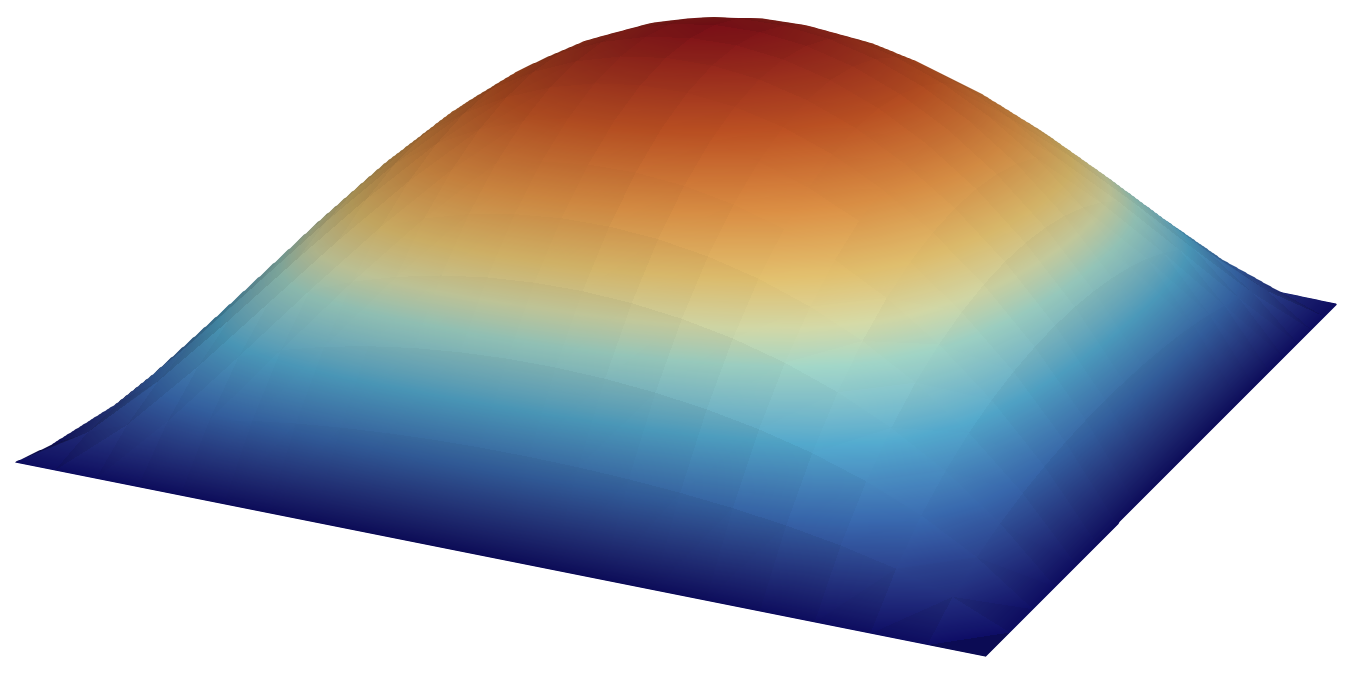
\includegraphics[width=5cm]{images/global-solution.png}};
    \node[inner sep=0] (topRectangle) at (topImg) 
        {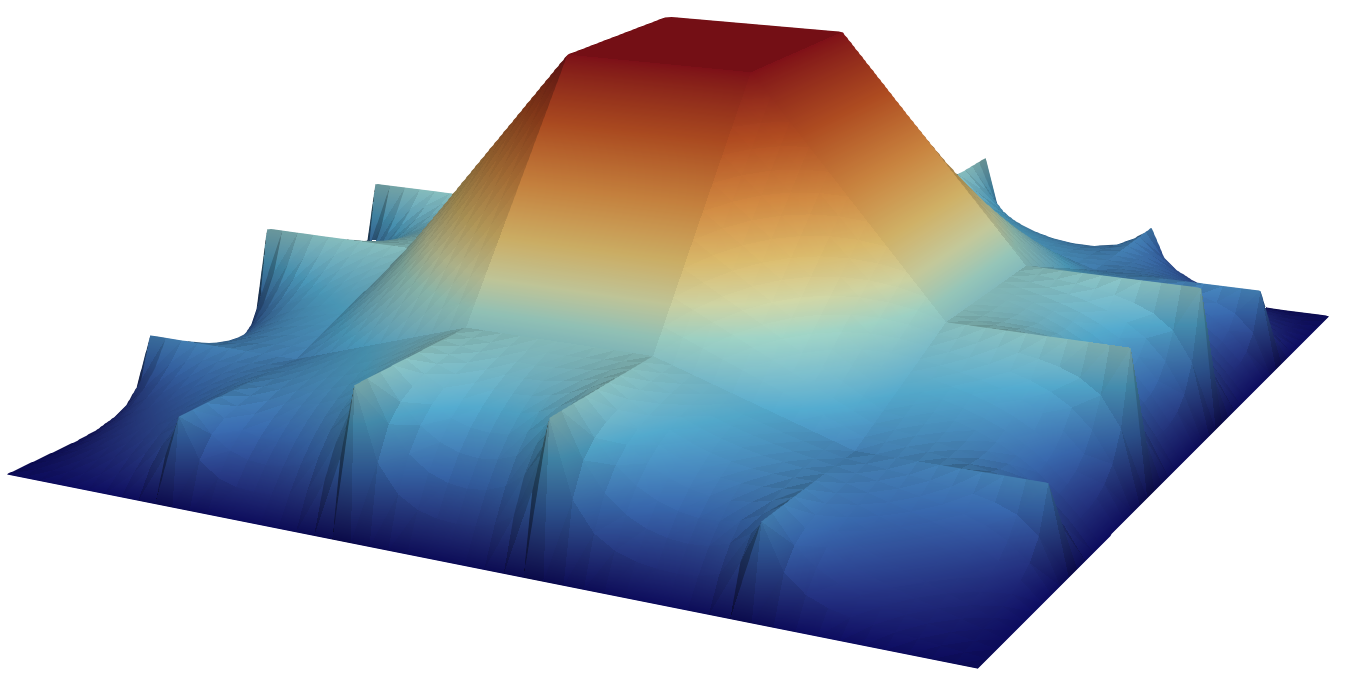
\includegraphics[width=5cm]{images/coarse-solution.png}};
     \node[inner sep=0] (bottomRectangle) at (bottomImg) 
        {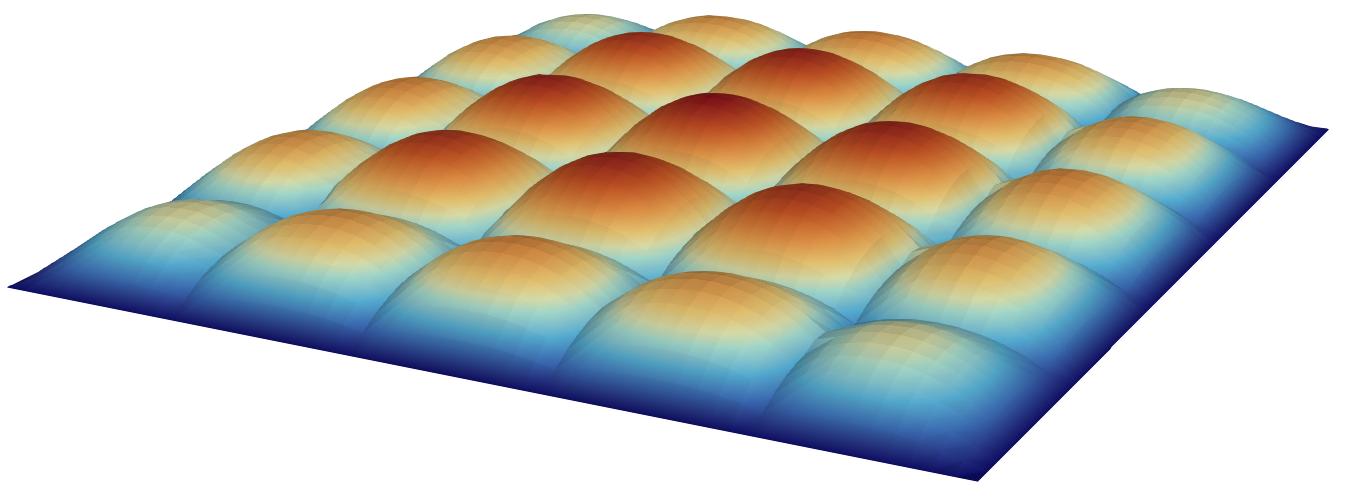
\includegraphics[width=5cm]{images/local-solutions.png}};
    
    \node[yshift=5mm, xshift=2mm, text width = 35mm, font=\small] at (leftRectangle.north) {Discretized nonlinear problem};
    \node[yshift=-2mm, font=\small] at (leftRectangle.south) {$F(u) = 0$};

    \node[yshift=-2mm, font=\small] at (bottomRectangle.south) {$R_i F\left(u - P_i T_i(u)\right) = 0$};
    
    \node [yshift=-2mm, font=\small] at (topRectangle.south){$R_0 F\left(u - P_0 T_0(u)\right) = 0$};
    
    \node[align=left, text width = 4.5cm, font=\small] at (9.6,-1.3){Solve with Newton's method for nonlinear corrections $T_i(u) \text{ for } i = 1,2,\dots,N$};
    
    \node[draw, rectangle, minimum width=4cm, minimum height=1cm, font=\small] (boxedEq) at (rightEq) {$\mathcal{F}(u) = \sum_{i=0}^{N} P_i T_i(u) = 0$};
    
    % Arrows
    \draw[-{Stealth[length=3mm, width=2mm]}] ($(leftRectangle.north east) + (-0.5, -0.5)$) -- ($(topRectangle.south west) + (0.3, 0.3)$);
    \draw[-{Stealth[length=3mm, width=2mm]}] ($(leftRectangle.south east) + (-0.7, 0.4)$) -- ($(bottomRectangle.north west) + (0.8, -0.2)$);
    \draw[-{Stealth[length=3mm, width=2mm]}] ($(topRectangle.south east)+ (-0.3, 0.7)$) -- ($(boxedEq.north west)+ (-0.1, 0.1)$);
    \draw[-{Stealth[length=3mm, width=2mm]}] ($(bottomRectangle.north east)+ (-0.8, -0.1)$) -- ($(boxedEq.south west)+ (-0.1, -0.1)$);
\end{tikzpicture}
